\documentclass[a4paper,12pt]{article}
\usepackage[french]{babel} 
\usepackage[T1]{fontenc}
%\usepackage[ansinew]{inputenc}
\usepackage[utf8]{inputenc}
\usepackage[top=3cm, bottom=3cm, left=2.3cm,right=2cm]{geometry}
\usepackage{graphicx}
\usepackage{color}
\usepackage{listings}
%\usepackage{marvosym}
%\usepackage{yfonts}
\usepackage[normalem]{ulem}
\usepackage{verbatim}
\usepackage{listings}
\usepackage{float}
%\renewcommand{\thesection}{\arabic{section}}
\usepackage{array} % pour les tableaux
\usepackage{amsmath} % pour les équations
\usepackage{float}
\usepackage{hyperref}	% crée des liens dans le pdf
\hypersetup{					% colorise les liens du pdf
  colorlinks=true,
  urlcolor=black
	citecolor=black,
  linkcolor=black,
  urlcolor=blue
}
\usepackage{url}			% change la police des url (utilisation : \url{http://asdf.ch})
\definecolor{dkgreen}{rgb}{0,0.6,0}
\definecolor{gray}{rgb}{0.5,0.5,0.5}
\definecolor{mauve}{rgb}{0.58,0.01,0.82}
%[babel=true]
\usepackage{csquotes}
\lstset{ %
  language=C,                % the language of the code
  basicstyle=\footnotesize,           % the size of the fonts that are used for the code
  numbers=left,                   % where to put the line-numbers
  numberstyle=\tiny\color{gray},  % the style that is used for the line-numbers
  stepnumber=1,                   % the step between two line-numbers. If it's 1, each line 
                                  % will be numbered
  numbersep=5pt,                  % how far the line-numbers are from the code
  backgroundcolor=\color{white},      % choose the background color. You must add \usepackage{color}
  showspaces=false,               % show spaces adding particular underscores
  showstringspaces=false,         % underline spaces within strings
  showtabs=false,                 % show tabs within strings adding particular underscores
  frame=single,                   % adds a frame around the code
  rulecolor=\color{black},        % if not set, the frame-color may be changed on line-breaks within not-black text (e.g. commens (green here))
  tabsize=2,                      % sets default tabsize to 2 spaces
  captionpos=b,                   % sets the caption-position to bottom
  breaklines=true,                % sets automatic line breaking
  breakatwhitespace=false,        % sets if automatic breaks should only happen at whitespace
  title=\lstname,                   % show the filename of files included with \lstinputlisting;
                                  % also try caption instead of title
  keywordstyle=\color{blue},          % keyword style
  commentstyle=\color{dkgreen},       % comment style
  stringstyle=\color{mauve},         % string literal style
  escapeinside={\%*}{*)},            % if you want to add a comment within your code
  morekeywords={*,...}               % if you want to add more keywords to the set
}

%Table of content with dot
\usepackage{etoolbox}
\makeatletter
\patchcmd{\l@section}
{\hfil}
{\leaders\hbox{\normalfont$\m@th\mkern \@dotsep mu\hbox{.}\mkern \@dotsep mu$}\hfill}
{}{}
\makeatother

%no indentation
\setlength{\parindent}{0cm}

%en-tête
\usepackage{fancyhdr}
\lhead{SEEE}
\chead{}
\rhead{\today}
\pagestyle{fancy}

% Title Page
\title{\Huge{\textsc{Systèmes d'exploitation et environnements d'exécution embarqués}} \\ 
	\Huge{\textbf{Rapport de laboratoire}} \\
	\huge{Master HES-SO}}
\author{Émilie \textsc{Gsponer}, Grégory \textsc{Emery} }
\date{\today \\
	version 1.0}

%-------------------------début du document-------------------------------------
\begin{document}

\maketitle % page de garde
\newpage
\tableofcontents % table des matières
\newpage
\section{Introduction REPTAR}
\subsection{Mise en place de l'environnement, utilisation de git}
\textbf{a) Donnée: }Il faut tout d'abord récupérer le dépôt étudiant pour les laboratoires SEEE à l'aide de la commande
suivante (via une fenêtre de terminal):
\begin{lstlisting}
$ git clone firstname.lastname@eigit.heig-vd.ch:/home2/reds/seee/seee_student
\end{lstlisting}
\textbf{Travail réalisé: }
Nous n'avions pas les droits d'accès pour le dépôt git, nous l'avons donc téléchargé, puis extrait depuis le lien:
\url{https://drive.switch.ch/index.php/s/TbHxQZtmO9IVdkb}.\\
Le dossier seee\_student a ensuite été placé dans: /home/redsuser/\\

\textbf{b) Donnée: }Lancez Eclipse et ouvrez le workspace seee\_student. Vous devriez obtenir la liste des projets (à
gauche). Chaque projet a un lien symbolique dans la racine du workspace. \\\\
\textbf{Travail réalisé: }
En introduisant le path du dossier seee\_student comme workspace au lancement d'Eclipse, nous obtenons la liste de projets suivante:
\begin{figure}[H]
	\begin{center}
		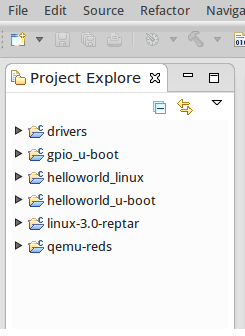
\includegraphics[height=7cm]{img/eclipseProjet.png}
		\caption{Liste des projets}
		\label{eclipseProjet}
	\end{center}
\end{figure}
\textbf{c) Donnée: }Compilez maintenant l'émulateur Qemu. Dans une fenêtre de terminal, lancez la commande
suivante à partir de votre répertoire seee\_student : 
\begin{lstlisting}
$ make qemu
\end{lstlisting}
\textbf{Travail réalisé: }
Vu que nous n'avons pas téléchargé le dossier de projets depuis git, il faut nettoyer le contenu du dossier avec clean ou distclean avant de pourvoir utiliser qemu. Le make qemu prend quelques instants.\\
\begin{lstlisting}
redsuser@vm-reds-2015s2:~/seee_student$ make clean
redsuser@vm-reds-2015s2:~/seee_student$ make qemu
...
make[1]: Leaving directory `/home/redsuser/seee_student/qemu-reds'
redsuser@vm-reds-2015s2:~/seee_student$
\end{lstlisting}
\subsection{Démarrage de Qemu}
\textbf{a) Donnée: }Depuis Eclipse, lancez le debugger avec la configuration de debug « qemu-reds Debug ». Dans la
fenêtre Console, vous pourrez entrer directement des commandes de U-boot (tapez help par
exemple). \\\\
\textbf{Travail réalisé: }
\begin{figure}[H]
	\begin{center}
		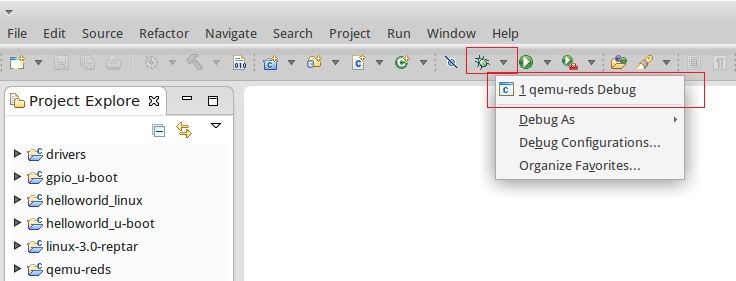
\includegraphics[height=7cm]{img/manip2Intro.png}
		\caption{Lancement d'Eclipse en mode Debug}
		\label{eclipseDebug}
	\end{center}
\end{figure}
\textbf{Remarque: }Après le lancement du Debug, il faut changer d'onglet en haut à droite en choisissant \textit{Debug} pour avoir la console. Ce changement d'onglet ne se fait pas automatiquement.
\begin{figure}[H]
	\begin{center}
		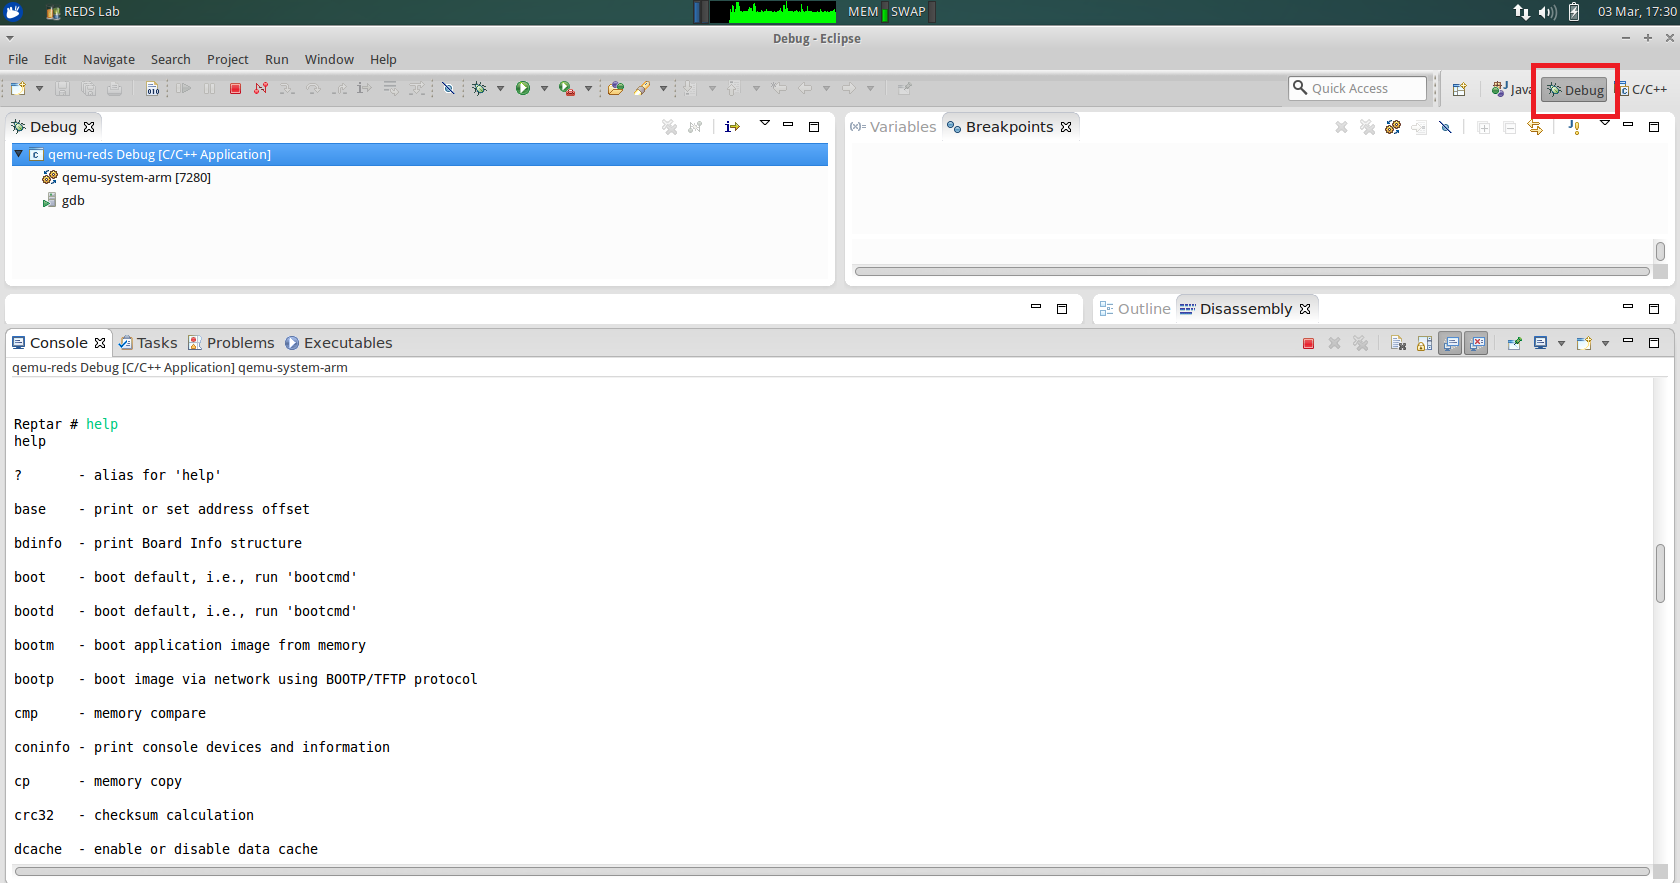
\includegraphics[width=18cm]{img/ubootCommand.png}
		\caption{Command help dans l'U-boot}
		\label{ubootCommand}
	\end{center}
\end{figure}
\textbf{b) Donnée: } Interrompez l'exécution du programme en cliquant sur l'icône pause. Identifiez la ligne en cours d'exécution dans le code source. \\\\
\textbf{Travail réalisé: }En interrompant le programme avec le bouton \textit{suspend}, on obtient la vue assembleur ci-dessous. L'environnement essaie d'ouvrir le fichier ppoll.c, on est donc en attente d'un événement. Le programme est interrompu après un syscall.
\begin{figure}[H]
	\begin{center}
		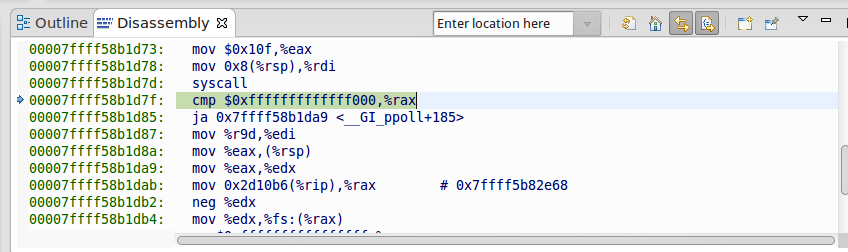
\includegraphics[width=18cm]{img/ubootAsm.png}
		\caption{Command help dans l'U-boot}
		\label{ubootAsm}
	\end{center}
\end{figure}
\textbf{c) Donnée: } Stoppez l'exécution, et dans une fenêtre de commande, démarrez qemu à l'aide du script stf (en
tapant ./stf) dans le répertoire racine. Vous arrivez dans U-boot. \\\\
\textbf{Travail réalisé: }Cette partie n'a plus rien avoir avec Eclipse, on peut le fermer et lancer un terminal.
Avec la commande \textit{stf} tapée à la racine du répertoire seee\_student, on arrive au même point qu'en lançant le Debug dans Eclipse. On peut également essayer la commande \textit{help}
\begin{lstlisting}
redsuser@vm-reds-2015s2:~/seee_student$ ./stf
WARNING: Image format was not specified for 'filesystem/flash' and probing guessed raw.
...

Reptar # help
?       - alias for 'help'
base    - print or set address offset
bdinfo  - print Board Info structure
boot    - boot default, i.e., run 'bootcmd'
bootd   - boot default, i.e., run 'bootcmd'
bootm   - boot application image from memory
bootp   - boot image via network usi
...
\end{lstlisting}
\subsection{Tests avec U-boot}
\textbf{a) Donnée: }Dans U-boot, listez les variables d'environnement avec la commande printenv. Observez les
variables prédéfinies « tftp1, tftp2 et goapp ». Ces variables définissent des commandes U-boot qui
peuvent être exécutées à l'aide de la commande run (par exemple run tftp1).
La commande go <addr> permet de lancer l'exécution à l'adresse physique <addr>.
Vous pouvez définir/modifier vos propres variables et les sauvegarder dans la flash émulée avec la
commande saveenv (seulement avec le lancement via stf). \\\\
\textbf{Travail Réalisé: }Après être entré dans l'U-boot avec \textit{stf}, nous avons pu lister les variables d'environnement suivantes:
\begin{lstlisting}
redsuser@vm-reds-2015s2:~$ cd seee_student/
redsuser@vm-reds-2015s2:~/seee_student$ ./stf
WARNING: Image format was not specified for 'filesystem/flash' and probing guessed raw.
...
goapp=go 0x81600000
...
tftp1=tftp helloworld_u-boot/helloworld.bin
tftp2=tftp gpio_u-boot/gpio_u-boot.bin

Environment size: 930/4092 bytes
Reptar # 
\end{lstlisting}
Les variables \textit{tftp1} et \textit{tftp2} sont des alias permettant de lancer des applications, la variable goapp est un alias permettant de lancer l'exécution de l'adresse physique 0x81600000. Elle définit l'adresse de début des applications. Voici un exemple d'utilisation de ces variables:
\begin{lstlisting}
redsuser@vm-reds-2015s2:~$ cd seee_student/
redsuser@vm-reds-2015s2:~/seee_student$ cd helloworld_u-boot/
redsuser@vm-reds-2015s2:~/seee_student/helloworld_u-boot$ make
...
redsuser@vm-reds-2015s2:~/seee_student/helloworld_u-boot$ cd ../gpio_u-boot/
redsuser@vm-reds-2015s2:~/seee_student/gpio_u-boot$ make
...
redsuser@vm-reds-2015s2:~/seee_student/gpio_u-boot$ cd ..
redsuser@vm-reds-2015s2:~/seee_student$ ./stf 
WARNING: Image format was not specified for 'filesystem/flash' and probing guessed raw.
...
Reptar # run tftp1
smc911x: detected LAN9118 controller
smc911x: phy initialized
smc911x: MAC e4:af:a1:40:01:fe
Using smc911x-0 device
TFTP from server 10.0.2.2; our IP address is 10.0.2.10
Filename 'helloworld_u-boot/helloworld.bin'.
Load address: 0x81600000
Loading: #
done
Bytes transferred = 776 (308 hex)

Reptar # run goapp
## Starting application at 0x81600000 ...
Example expects ABI version 6
Actual U-Boot ABI version 6
Hello World
argc = 1
argv[0] = "0x81600000"
argv[1] = "<NULL>"
Hit any key to exit ... 
## Application terminated, rc = 0x0

Reptar # run tftp2
smc911x: detected LAN9118 controller
smc911x: phy initialized
smc911x: MAC e4:af:a1:40:01:fe
Using smc911x-0 device
TFTP from server 10.0.2.2; our IP address is 10.0.2.10
Filename 'gpio_u-boot/gpio_u-boot.bin'.
Load address: 0x81600000
Loading: #
done
Bytes transferred = 3080 (c08 hex)

Reptar # run goapp
## Starting application at 0x81600000 ...
Start of the GPIO U-boot Standalone Application
Stop of the GPIO U-boot Standalone Application
## Application terminated, rc = 0x0
Reptar #
\end{lstlisting}
La commande run tftp<x> charge une application à l'adresse 0x81600000, tandis que run goapp va exécuter l'application à cette adresse comme le montre l'exemple ci-dessus.\\\\
\textbf{b) Donnée: }La production de l'exécutable helloworld\_u-boot s'effectue en tapant la commande make dans le
répertoire contenant les sources du programme. Ensuite, vous pouvez transférer le fichier (extension
.bin) dans U-boot et exécuter le binaire (aidez-vous des variables d'environnement prédéfinies). \\\\
\textbf{Travail réalisé: } Ce point a été fait en même temps que le précédent.\\

\textbf{c) Donnée: } Testez le debugger dans Eclipse avec le projet helloworld\_u-boot. Mettez un breakpoint dans le
code source au démarrage du programme, et lancez le debugger avec la configuration de debug
« helloworld\_u-boot Debug ». \\\\
\textbf{Travail Réalisé: } Il faut que U-boot soit démarré dans un terminal externe avec \textit{stf} pour que la manipulation fonctionne avec Eclipse.
\begin{figure}[H]
	\begin{center}
		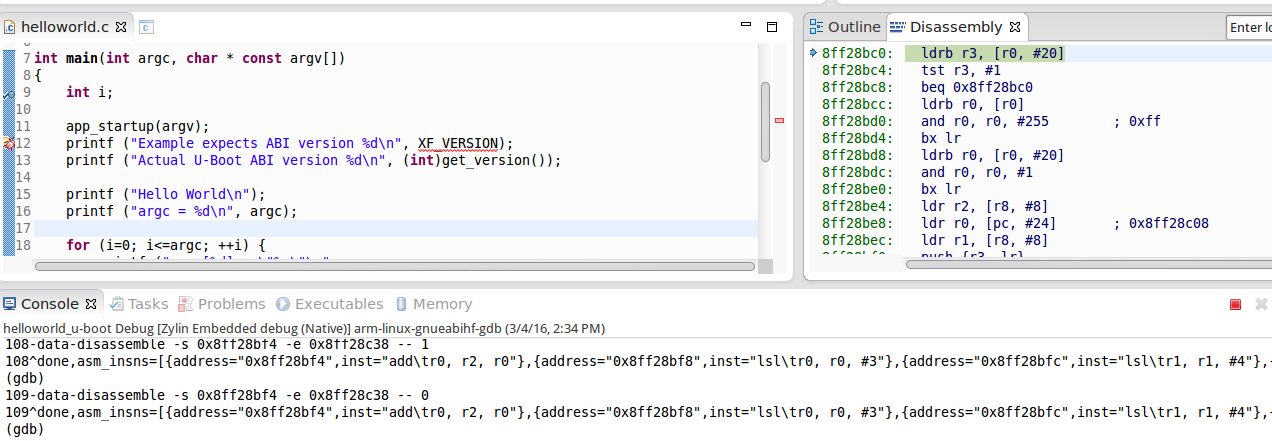
\includegraphics[width=18cm]{img/ubootCommand2.png}
		\caption{Debug d'hello\_world\_u-boot}
		\label{ubootComm2}
	\end{center}
\end{figure}
\textbf{Remarque: }\color{red}Qemu se comporte comme un serveur GDB, ce qui permet à Eclipse  de communiquer avec lui et de debugger des applications...à retravailler\color{black}
\subsection{Tests avec Linux}
\textbf{a) Donnée: }Lancez le script ./deploy qui permettra de déployer le noyau Linux dans la sdcard virtuelle (ignorez
l'erreur due à l'absence de certains fichiers). \\\\
\textbf{Travail réalisé: }
\begin{lstlisting}
redsuser@vm-reds-2015s2:~/seee_student$ ./deploy 
Deploying into reptar rootfs ...
Mounting filesystem/sd-card.img...
[sudo] password for redsuser: 
SD card partitions mounted in 'boot_tmp' and 'filesystem_tmp' directories
cp: cannot stat 'drivers/sp6.ko': No such file or directory
cp: cannot stat 'drivers/usertest': No such file or directory
cp: cannot stat 'drivers/buttons_test': No such file or directory
Unmounting SD card image...
Synchronizing .img file
Unmounting 'boot_tmp' and 'filesystem_tmp'...
Done !
redsuser@vm-reds-2015s2:~/seee_student$ 
\end{lstlisting}
\textbf{b) Donnée: }Poursuivez ensuite en cross-compilant l'application helloworld pour Linux (via make). \\\\
\textbf{Travail réalisé: }
\begin{lstlisting}
redsuser@vm-reds-2015s2:~/seee_student$ cd helloworld_linux/
redsuser@vm-reds-2015s2:~/seee_student/helloworld_linux$ make
...
redsuser@vm-reds-2015s2:~/seee_student/helloworld_linux$ cd ..
\end{lstlisting}
\textbf{c) Donnée: }Copiez l'exécutable dans le rootfs\\\\
\textbf{Travail réalisé: }
\begin{lstlisting}
redsuser@vm-reds-2015s2:~/seee_student$ ./mount-sd.sh 
Mounting filesystem/sd-card.img...
SD card partitions mounted in 'boot_tmp' and 'filesystem_tmp' directories

redsuser@vm-reds-2015s2:~/seee_student$ sudo cp helloworld_linux/helloworld filesystem_tmp/root

redsuser@vm-reds-2015s2:~/seee_student$ ./umount-sd.sh 
Unmounting SD card image...
Synchronizing .img file
Unmounting 'boot_tmp' and 'filesystem_tmp'...
Done !
redsuser@vm-reds-2015s2:~/seee_student$ 
\end{lstlisting}
\textbf{d) Donnée: }Lancez le script stq suivi de la commande boot dans U-boot pour amorcer le démarrage de Linux\\\\
\textbf{Travail réalisé: } Avec la commande stq, une représentation de la carte se lance.
\begin{lstlisting}
redsuser@vm-reds-2015s2:~/seee_student$ ./stq 
libGL error: failed to authenticate magic 1
libGL error: failed to load driver: vboxvideo
Running QEMU
...
Warning: smc911x-0 MAC addresses don't match:
Address in SROM is         52:54:00:12:34:56
Address in environment is  e4:af:a1:40:01:fe
Reptar # boot
reading uImage
...
*** Welcome on REPTAR (HEIG-VD/REDS): use root/root to log in ***
reptar login: root
Password: 
# 
\end{lstlisting}
\begin{figure}[H]
	\begin{center}
		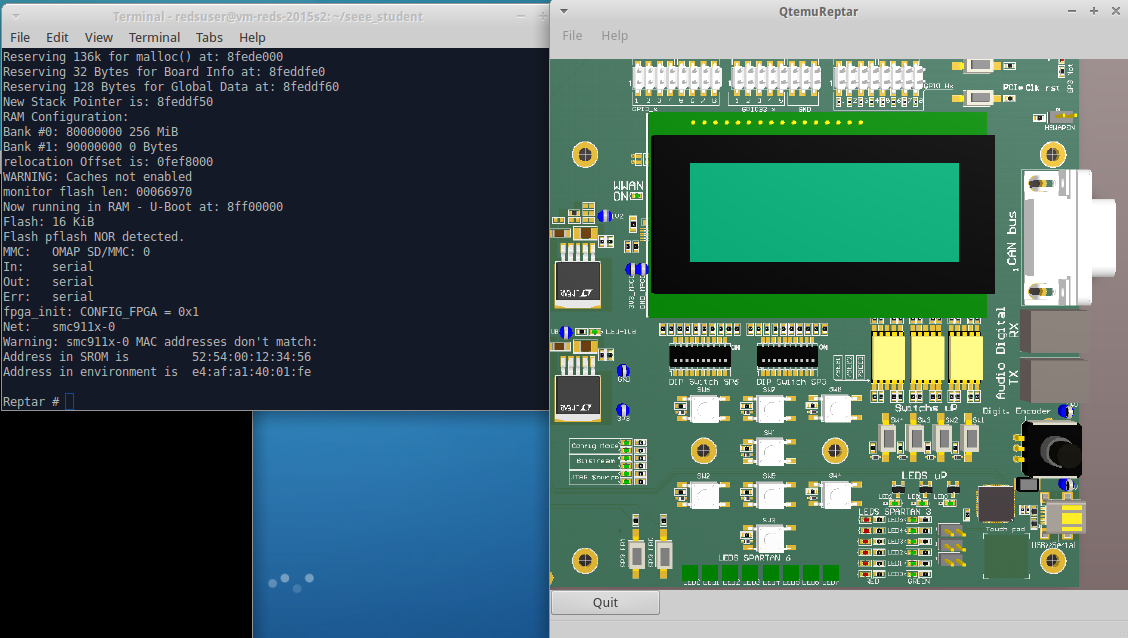
\includegraphics[width=18cm]{img/linux.png}
		\caption{Environnement émulé}
		\label{linux}
	\end{center}
\end{figure}
\textbf{e) Donnée: }Lancez votre application\\\\
\textbf{Travail réalisé: }
\begin{lstlisting}
# ls
Settings         fs               helloworld       rootfs_domU.img
# ./helloworld 
Hello world within Linux
argv[0] = ./helloworld
# 
\end{lstlisting}
\textbf{f) Donnée: }Dans Linux, tapez la commande suivante :
\begin{lstlisting}
$ /usr/share/qt/examples/effects/lighting/lighting -qws & 
\end{lstlisting}
\textbf{Travail réalisé: }Cette commande permet de lancer une application pré installée de l'émulateur.
\begin{figure}[H]
	\begin{center}
		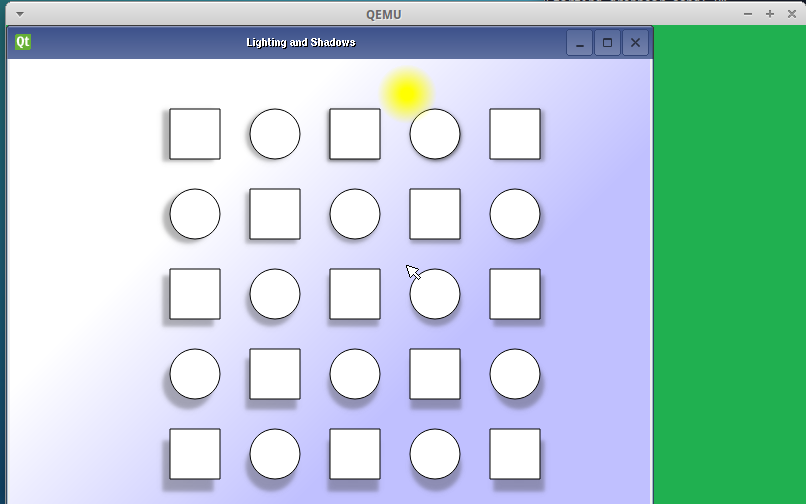
\includegraphics[width=10cm]{img/linux2.png}
		\caption{Lancement d'une application}
		\label{linux2}
	\end{center}
\end{figure}
\subsection{Tests sur la plate-forme réelle}
\textbf{a) Donnée: }Déployez l'application helloworld dans U-boot sur la plate-forme REPTAR avec l'interface réseau.
Le transfert peut s'effectuer avec la commande tftp.
Il est nécessaire d’exécuter la commande suivante pour mettre à jour les adresses IP et MAC de la plate-forme
REPTAR : 
\begin{lstlisting}
# run setmac setip 
\end{lstlisting}
\textbf{Travail réalisé: }Avec la commande tftp il faut donner comme paramètre le \textit{.bin} de l'application ainsi que l'adresse physique où charger le programme. Cette adresse est 0x81600000 comme dans les exercices précédents.
\begin{lstlisting}
redsuser@vm-reds-2015s2:~/seee_student$ cd helloworld_u-boot/
redsuser@vm-reds-2015s2:~/seee_student/helloworld_u-boot$ make
redsuser@vm-reds-2015s2:~/seee_student/helloworld_u-boot$ cp helloworld.bin /home/redsuser/tftpboot
redsuser@vm-reds-2015s2:~/seee_student/helloworld_u-boot$ sudo picocom -b 115200 /dev/ttyUSB0 
[sudo] password for redsuser: 
picocom v1.7
...
Terminal ready

Reptar # run setmac setip
Reptar # tftp 0x81600000 helloworld.bin
smc911x: detected LAN9220 controller
smc911x: phy initialized
smc911x: MAC e4:af:a1:40:01:fe
Using smc911x-0 device
TFTP from server 192.168.1.1; our IP address is 192.168.1.254
Filename 'helloworld.bin'.
Load address: 0x81600000
Loading: T #
done
Bytes transferred = 776 (308 hex)

Reptar # go 0x81600000
## Starting application at 0x81600000 ...
Example expects ABI version 6
Actual U-Boot ABI version 6
Hello World
argc = 1
argv[0] = "0x81600000"
argv[1] = "<NULL>"
Hit any key to exit ... 
\end{lstlisting}
\textbf{Remarque: }La commande tftp ne fonctionnera pas tant que la configuration réseau n'est pas correcte. Il faut impérativement que l'adresse Ip de la connexion par pont de la VM soit 192.168.1.1.
\begin{figure}[H]
	\begin{center}
		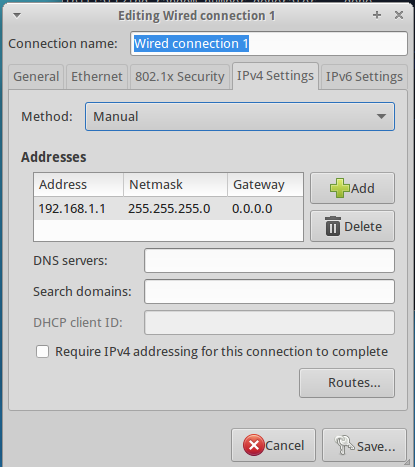
\includegraphics[width=10cm]{img/ipConfig.png}
		\caption{Configuration réseau}
		\label{ipConfig}
	\end{center}
\end{figure}
\textbf{b) Donnée: }Déployez l'application helloworld dans Linux à l'aide du réseau et de la commande scp.\\\\
\textbf{Travail réalisé: } Nous avons découvert que l'adresse Ip de la carte n'était pas celle attendue, nous avons donc dû adapter scp pour l'adresse Ip 192.168.1.254.
\begin{lstlisting}
Reptar # boot
reading uImage
...
*** Welcome on REPTAR (HEIG-VD/REDS): use root/root to log in ***
reptar login: root
Password: 
# ifconfig
eth0      Link encap:Ethernet  HWaddr E4:AF:A1:40:01:FE  
inet addr:192.168.1.254  Bcast:192.168.1.255  Mask:255.255.255.0
...
\end{lstlisting}
La commande scp permet de transférer le helloworld\_linux à la carte reptar par l'interface réseau depuis la machine hôte.
\begin{lstlisting}
redsuser@vm-reds-2015s2:~/seee_student/helloworld_linux$ scp helloworld root@192.168.1.254:helloworld

The authenticity of host '192.168.1.254 (192.168.1.254)' can't be established.
RSA key fingerprint is fb:59:a3:73:97:9d:b7:b9:8a:40:e8:bc:19:ab:ab:70.
Are you sure you want to continue connecting (yes/no)? yes
Warning: Permanently added '192.168.1.254' (RSA) to the list of known hosts.
root@192.168.1.254's password: 
helloworld                                    100% 6877     6.7KB/s   00:00    
\end{lstlisting}
L'application helloworld est maintenant chargée sur la cible, il ne reste plus qu'à l'exécuter sur celle-ci.
\begin{lstlisting}
# ls
bitstreams  helloworld     tests
# ./helloworld 
Hello world within Linux
argv[0] = ./helloworld
#
\end{lstlisting}
\subsection{Accès aux périphériques REPTAR}
\textbf{a) Donnée: } Sur la base de l’exemple gpio\_u-boot., vous devez développer une application permettant d’interagir avec les
LEDs et les switchs présents sur la carte CPU de la plate-forme REPTAR.
Le but de l’application est d’allumer une LED lorsqu’on appuie sur un switch.
\begin{enumerate}
	\item La LED 0 doit s’allumer lorsqu’on appuie sur le SWITCH 0.
	\item La LED 1 s’allume si l’on appuie sur le SWITCH 1.
	\item Et ainsi de suite pour les LEDs et switchs 0..3 de la carte CPU.
\end{enumerate}
Le switch numéro 4 sert à quitter l’application. Aidez-vous des fichiers d'en-tête (\#include) déjà présents dans
le chablon fourni.\\
L’application gpio\_u-boot est à déployer dans U-boot via la commande tftp. \\\\
\textbf{Emplacement du code réalisé: }/gpio\_u-boot.c\\\\
Ce code est très basique, mais implémente correctement les points exigés par la donnée. Les commandes suivantes ont permis de lancer l'application sur la cible réelle dans l'U-boot. Une pression sur le switch numéro 4 permet de terminer l'application.\\
\begin{lstlisting}
redsuser@vm-reds-2015s2:~/seee_student/gpio_u-boot$ make
...
redsuser@vm-reds-2015s2:~/seee_student/gpio_u-boot$ cp gpio_u-boot.bin /home/redsuser/tftpboot
redsuser@vm-reds-2015s2:~/seee_student/gpio_u-boot$ sudo picocom -b 115200 /dev/ttyUSB0 
[sudo] password for redsuser: 
picocom v1.7
...
Terminal ready

Reptar # tftp 0x81600000 gpio_u-boot.bin
smc911x: detected LAN9220 controller
smc911x: phy initialized
smc911x: MAC e4:af:a1:40:01:fe
Using smc911x-0 device
TFTP from server 192.168.1.1; our IP address is 192.168.1.254
Filename 'gpio_u-boot.bin'.
Load address: 0x81600000
Loading: T #
done
Bytes transferred = 776 (308 hex)

Reptar # go 0x81600000
...
Stop of the GPIO U-boot Standalone Application
Reptar #
\end{lstlisting}

\end{document}


